
\documentclass{beamer}

\usepackage{algpseudocode, color, colortbl}

\usepackage{hyperref}
\hypersetup{
    colorlinks=true,
    urlcolor=blue,
}

\usetheme{Montpellier}
\usecolortheme{rose}

% page numbers, from
% https://tex.stackexchange.com/questions/137022/how-to-insert-page-number-in-beamer-navigation-symbols
\expandafter\def\expandafter\insertshorttitle\expandafter{%
  \insertshorttitle\hfill%
  \insertframenumber\,/\,\inserttotalframenumber}

\definecolor{Gray}{gray}{0.8}
\newcolumntype{g}{>{\columncolor{Gray}}c}

\newcommand{\stanza}{ \\~\ }

\title{09. Linear Programming Formulations}
\subtitle{CPSC 535}
\author{Kevin A. Wortman}
\institute{ 
\includegraphics[height=2cm]{csuf-logo-cmyk} }
\date{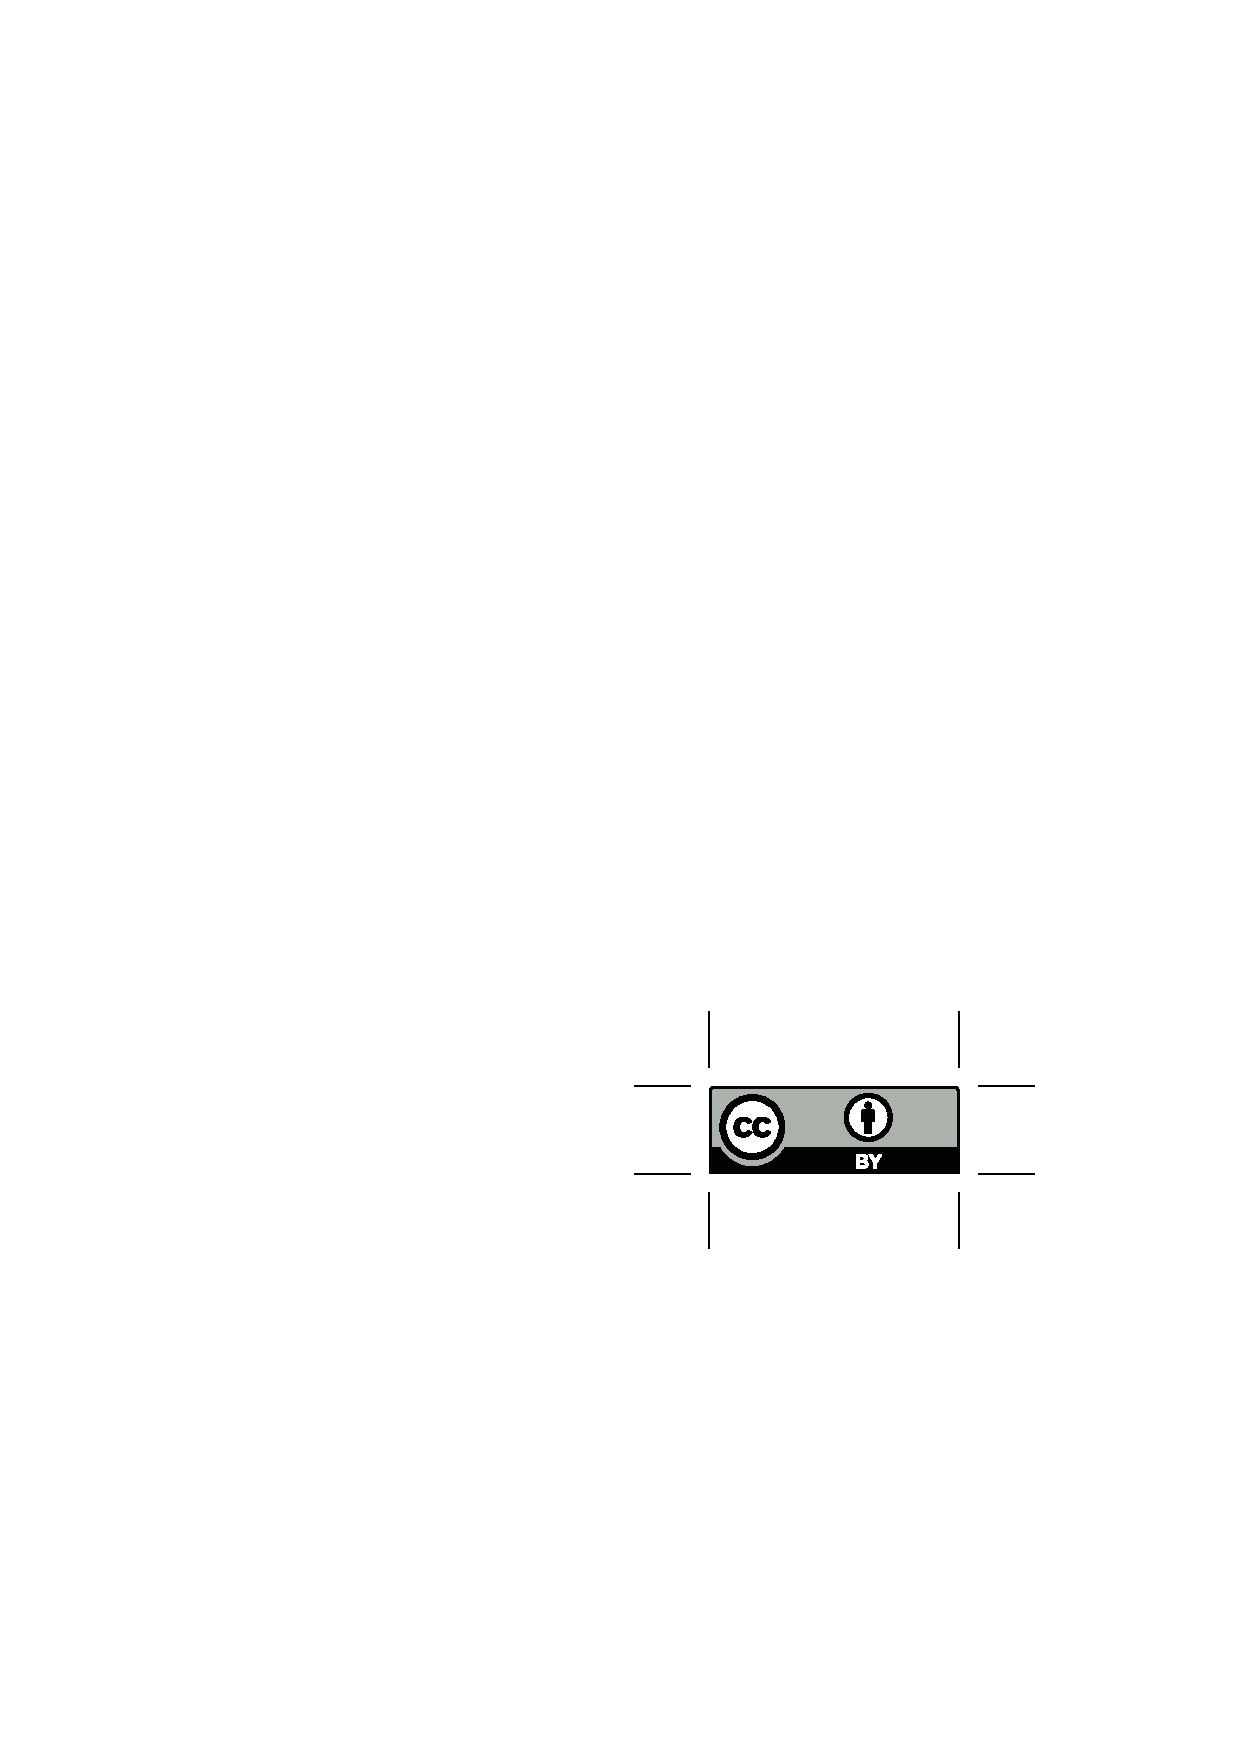
\includegraphics[height=14pt]{by} \\

{\tiny
This work is licensed under a
\href{http://creativecommons.org/licenses/by/4.0/}{Creative Commons Attribution 4.0 International License}.
}}

\begin{document}

\begin{frame}
  \titlepage
\end{frame}

\begin{frame} \frametitle{Linear Programming Formulations}
  Many problems reduce to standard-form linear programming (LP):
  \begin{itemize}
    \item generalize standard form to be more flexible
    \begin{itemize}
      \item allow minimization, negative variables, $=$ constraints, $\geq$ constraints
    \end{itemize}
    \item business/administrative problems (``operations research'')
    \item problems that don't resemble LP: shortest paths, max flow
    \item (similar situation to max-flow formulations)
  \end{itemize}
\end{frame}

\begin{frame} \frametitle{Standard Form versus General Form}
\textbf{general form LP:} a ``real'' LP, more flexible than standard form (previous slides)
\begin{center}
  \begin{tabular}{|l|l|}
    \hline
    \textbf{Standard Form} & \textbf{General Form} \\ \hline
    maximize objective function & maximize \textbf{or minimize} obj. func. \\ \hline
    all variables are non-negative & no restriction (may be negative) \\ \hline
    every constraint is $\leq$ r.h.s. & constraint may be $=$ or $\geq$ r.h.s. \\ \hline
  \end{tabular}
\end{center}
\end{frame}

\begin{frame} \frametitle{Standard Form Example}
  maximize $2 x_1 + x_2 - \frac{1}{3} x_3$ \\
  subject to
  \begin{eqnarray*}
  x_1 + x_2 &\leq& 10 \\
  -x_3 &\leq& -2 \\
  x_1, x_2, x_3 &\geq& 0
  \end{eqnarray*}
\end{frame}

\begin{frame} \frametitle{General Form Example}
  minimize $x_1 - x_2 + \ldots + c_n x_n$ \\
  subject to
  \begin{eqnarray*}
    x_1 &\leq& 100 \\
    x_2 &\geq& 2 \\
    x_1 + x_2 &=& 10 \\
    x_2 &\geq& 0
  \end{eqnarray*}

Note
\begin{itemize}
  \item minimizing objective function
  \item mix of $\leq, =, \geq$ constraints
  \item not all variables have $x_i \geq 0$ non-negativity constraint ($x_1$ is missing)
\end{itemize}
\end{frame}

\begin{frame} \frametitle{Formulating General LP as Standard LP}
  \begin{itemize}
    \item pre-processing: convert general LP to standard LP
    \item need to get rid of any non-standard feature
    \item want insignificant overhead
    \begin{itemize}
      \item $n = $ \#variables, $m = $ \# constraints
      \item space complexity of general LP is $\Theta(nm)$
      \item want size of resulting standard LP, and time overhead, to both be
      $O(nm)$
    \end{itemize}
    \item three features to deal with
    \begin{itemize}
      \item minimization
      \item negative variables
      \item $=, \geq$ constraints
    \end{itemize}
  \end{itemize}
\end{frame}

\begin{frame} \frametitle{Converting ``minimize'' to Standard Form}
  \begin{itemize}
    \item minimize $f(x) \equiv$ maximize $-f(x)$
    \item so if general LP says
    \[ \text{minimize } c_1 x_1 + c_2 x_2 + \ldots + c_n x_n \]
    \item replace that with
    \[ \text{maximize } -c_1 x_1 - c_2 x_2 - \ldots - c_n x_n \]
    \item size of $LP$ unchanged
    \item $O(n)$ time to negate coefficients
  \end{itemize}
\end{frame}

\begin{frame} \frametitle{Converting Negative Variables to Standard Form}
The idea:
  \begin{itemize}
    \item if $x_j$ does not have a non-negativity constraint $x_j \geq 0$,
      call $x_j$ a \emph{negative variable}
    \item handle each negative variable one at a time
    \item negative variable $x_j$ becomes two non-negative variables $x_j', x_j''$
    \item invariant: $x_j = x_j'-x_j''$
    \item $x_j' = $ the ``positive'' part of $x_j$
    \item $x_j'' = $ the ``negative'' part of $x_j$
    \item $x_j $ positive $\Longleftrightarrow$ $x_j'>0, x_j''=0$
    \item $x_j $ negative $\Longleftrightarrow$ $x_j'=0, x_j''>0$
  \end{itemize}
\end{frame}

\begin{frame} \frametitle{Converting Negative Variables to Standard Form}
  The algorithm:
  \begin{itemize}
    \item add non-negativity constraints $x_j' \geq 0, x_j'' \geq 0$
    \item substitute $(x_j'-x_j'')=x_j$ into LP
    \begin{itemize}
      \item obj. func: $c_j x_j \Rightarrow c_j(x_j'-x_j'')=c_j x_j' - c_j x_j''$
      \item constraints: $a_{i,j} x_j \Rightarrow a_{i,j} (x_j'-x_j'') = a_{i, j} x_j' - a_{i, j} x_j''$
    \end{itemize}
    \item after solving standard LP, to complete general LP evaluate $x_j=x_j'-x_j''$
    \item $n, m$ at most double $\Rightarrow$ still $\Theta(nm)$ space
    \item $O(nm)$ time with care (do all substitutions in one pass)
  \end{itemize}
\end{frame}

\begin{frame} \frametitle{Converting $=$ Constraints to Inequalities}
  \begin{itemize}
    \item this step converts any $=$ constraint to $\leq, \geq$ constraints
    \item $\geq$ constraints are eliminated in the next step
    \item $a = b \Longleftrightarrow a \leq b \text{ and } a \geq b$
    \item replace each $=$ constraint
    \[ a_{i, 1} x_1 + a_{i, 2} x_2 + \ldots + a_{i, n} x_n = b_n \]
    with two constraints
    \[ a_{i, 1} x_1 + a_{i, 2} x_2 + \ldots + a_{i, n} x_n \geq b_n \]
    \[ a_{i, 1} x_1 + a_{i, 2} x_2 + \ldots + a_{i, n} x_n \leq b_n \]
    \item $n$ unchanged, $m$ at most doubles $\Rightarrow$ still $\Theta(nm)$ space
    \item $O(nm)$ time
  \end{itemize}
\end{frame}

\begin{frame} \frametitle{Converting $\geq$ Constraints to $\leq$}
  \begin{itemize}
    \item $a \geq b \Longleftrightarrow -a \leq -b$
    \item replace each $\geq$ constraint
    \[ a_{i, 1} x_1 + a_{i, 2} x_2 + \ldots + a_{i, n} x_n \geq b_n \]
    with
    \[ -a_{i, 1} x_1 - a_{i, 2} x_2 - \ldots - a_{i, n} x_n \leq -b_n \]
    \item $n, m$ unchanged so still $\Theta(nm)$ space
    \item $O(nm)$ time
\end{itemize}
\end{frame}

\begin{frame} \frametitle{General LP Problem}
  \emph{general-form linear programming problem} \\
  \textbf{input:}
  \begin{itemize}
    \item Boolean for whether $f$ is maximized/minimized
    \item vector $c \in \mathbb{R}^n$
    \item vector $b \in \mathbb{R}^m$
    \item vector $o \in \{\leq, =, \geq\}^m$
    \item $m \times n$ matrix $A$ of real numbers
  \end{itemize}
  \textbf{output:} one of
  \begin{enumerate}
    \item ``unbounded'';
    \item ``infeasible''; or
    \item ``solution'' with a vector $x \in \mathbb{R}^n$
      maximizing the objective function
  \end{enumerate}
\end{frame}

\begin{frame} \frametitle{Time Complexity}
  \begin{itemize}
    \item converting a general-form LP to standard-form takes $\Theta(nm)$
    time
    \item so time to solve general LP is
    \[ O(nm + \text{time to solve standard LP}) \]
    \item standard-LP solver needs to spend at least $\Omega(nm)$ time
      just to read in the input
    \item $\Rightarrow$ time to solve general LP = $O(\text{time to solve standard LP})$
    (w/ worse constant factors)
    \item from now on we will formulate general LPs
  \end{itemize}
\end{frame}

\begin{frame} \frametitle{Formulating General LPs}
  Need to define
  \begin{enumerate}
    \item the variables, \textbf{what they represent}
    \item the objective function, whether it is maximize or minimize
    \item the constraints, \textbf{what they represent}
    \item the entire LP in general form
    \item how to interpret
    \begin{itemize}
      \item infeasible result
      \item unbounded result
      \item solution result; how to interpret solution vector $x$ in
        terms of business logic
    \end{itemize}
  \end{enumerate}
\end{frame}

\begin{frame} \frametitle{Formulating Business Logic}
  \begin{itemize}
    \item business scenario is a ``word problem'' that defines business-logic
      rules, resource limits, what needs to be optimized
    \item you need to figure out how to model all these in parts of an LP
    \begin{itemize}
      \item variables
      \item objective function
      \item constraints
    \end{itemize}
    \item every concept mentioned in the scenario needs to be modeled in the LP somehow
    \item only works when the objective is a linear function (not squared, exponential, etc.)
  \end{itemize}
\end{frame}

\begin{frame} \frametitle{Example: Plastic Recycling}
  Suppose Orange County has the following options for disposing of plastic waste:
  \begin{center}
  \begin{tabular}{lll}
    \textbf{Method} & \textbf{Carbon/ton} & \textbf{Dollars/ton} \\
    Local incinerator & 2.9 & 800 \\
    Overseas incinerator & 3.2 & 600 \\
    Thermal recycling & .5 & 1200 \\
    Landfill & .3 & 1400 \\
  \end{tabular}
\end{center}
  November is expected to produce 700 tons of plastic and is required by law
  to emit no more than 1400 tons of carbon. The landfill can accommodate up
  to 100 tons per month and the other methods are effectively unlimited.
  The County Supervisors want you to minimize the cost of plastic disposal.
\end{frame}

\begin{frame} \frametitle{Example: Plastic Recycling}
\begin{enumerate}
  \item \textbf{Variables:} create a variable to represent how much of each
    method to use,
    \begin{eqnarray*}
      I &\equiv& \text{ tons incinerated locally } \\
      O &\equiv& \text{ tons incinerated overseas } \\
      R &\equiv& \text{ tons recycled } \\
      L &\equiv& \text{ tons sent to landfill } \\
    \end{eqnarray*}
  \item \textbf{Objective function:}
  \begin{itemize}
    \item ``County Supervisors want you to minimize the cost''
    \[ \text{ minimize } 800I + 600O + 1200R + 1400L \]
  \end{itemize}
\end{enumerate}
\end{frame}

\begin{frame} \frametitle{Example: Plastic Recycling}
\begin{enumerate}
  \setcounter{enumi}{2}
  \item \textbf{Constraints:}
  \begin{itemize}
    \item re-read the word problem and pick out rules
    \item ``produce 700 tons of plastic'': \[I+O+R+L=700\]
    \item ``no more than 1400 tons of carbon'': \[2.9I + 3.2O + .5R + .3L \leq 1400\]
    \item ``landfill can accommodate up to 100 tons'': \[L \leq 100\]
    \item also, use critical thinking, common sense to model implicit rules
    \[ I, O, R, L \geq 0 \]
  \end{itemize}
\end{enumerate}
\end{frame}

\begin{frame} \frametitle{Example: Plastic Recycling}
  \begin{enumerate}
    \setcounter{enumi}{3}
\item general-form LP: \stanza

minimize $800I + 600O + 1200R + 1400L$ \\
subject to
\begin{eqnarray*}
  I+O+R+L &=& 700 \\
  2.9I + 3.2O + .5R + .3L &\leq& 1400 \\
  L &\leq& 100 \\
  I, O, R, L &\geq& 0 \\
\end{eqnarray*}
\end{enumerate}
\end{frame}

\begin{frame} \frametitle{Example: Plastic Recycling}
\begin{enumerate}
  \setcounter{enumi}{4}
  \item \textbf{Interpret results:}
  \begin{itemize}
    \item infeasible: never happens because there exists at least one feasible
      solution: $R=700, I=O=L=0$
    \item unbounded: never happens because the
      non-negativity constraints lower-bound the objective at 0; it can't
      approach $-\infty$
    \item solution: Tell the Supervisors to incinerate $I$ tons locally,
    incinerate $O$ tons overseas, recycle $R$ tons, and landfill $L$ tons.
  \end{itemize}
\end{enumerate}
\end{frame}

\begin{frame} \frametitle{Single-Source Shortest Paths}
  \emph{single-source single-sink shortest paths (1S1SSP) problem} \\
  \textbf{input:} weighted undirected graph $G=(V,E),$ source vertex $s \in V$,
    sink vertex $t \in V$\\
  \textbf{output:} the shortest path $s \leadsto t$ in $G$ \stanza

  \begin{itemize}
    \item Bellman-Ford algorithm solves this in $\Theta(|V| \cdot |E|)$ time
    \item when every weight $w(e) \geq 0,$ Dijkstra's algorithm solves this
      in $\Theta(|E| + |V| \log |V|)$ time
  \end{itemize}
\end{frame}

\begin{frame} \frametitle{Formulating Single-Source Shortest Paths}
\begin{enumerate}
  \item \textbf{Variables:} for each vertex $v \in V,$ create an LP variable
  \[ d_v \equiv \text{ total weight of shortest path } s \leadsto v \text{ in } G \]
  \item \textbf{Objective function:} hold that thought
  \item \textbf{Constraints:}
  \begin{itemize}
    \item Recall that in Bellman-Ford and Dijkstra, we compute
    \[ d_v = \min_{x \in V, \{x, v\} \in E} d_x + w({x, v}) \]
    \item LP can't express ``min'' but we can say $d_v \leq$ every candidate:
    \[ d_v \leq d_x + w(\{x, v\}) \qquad \forall x \in V, \{x, v\} \in E \]
    \item $d_s = 0$ because it is the source
  \end{itemize}
\end{enumerate}
\end{frame}

\begin{frame} \frametitle{Formulating Single-Source Shortest Paths}
\begin{enumerate}
  \setcounter{enumi}{1}
  \item \textbf{Objective function:} for sink $t,$ maximize $d_t$
\begin{itemize}
  \item \emph{not} minimize $d_t$
  \item that would allow LP to just set every $d_v = 0$; no notion of
    edges adding to path weights
  \item maximizing $d_t$ forces LP to set each $d_v$ to the
    $d_x + w(\{x, v\})$ that is the minimum
  \item now, when you use an edge, you add its weight
\end{itemize}
\setcounter{enumi}{3}
\item \textbf{General-form LP:} given $G=(V, E)$, source $s,$ sink $t$ \\
create variable $d_v \enspace \forall v \in V$ \\
maximize $d_t$ \\
subject to
\begin{eqnarray*}
  d_v &\leq& d_x + w(x, v) \qquad \forall \{x, v \} \in E \\
  d_s &=& 0
\end{eqnarray*}
\end{enumerate}
\end{frame}

\begin{frame} \frametitle{Formulating Single-Source Shortest Paths}
  \begin{enumerate}
    \setcounter{enumi}{4}
    \item \textbf{Interpreting result:}
    \begin{itemize}
      \item infeasible: never happens because setting every $d_v=0$ is always feasible
      \item unbounded: $d_t = \infty$ means that $t$ is unreachable from $s$
      \item solution:
      \begin{itemize}
        \item need to identify path (list of vertices) $s \leadsto t$
        \item i.e. identify edges definining the shortest path and $d_t$
        \item find the constraints where
        \[ d_v = d_x + w(x, v) \]
        (not $<$); these vertices $x, v$ are part of the shortest path
        \item use BFS or DFS, limited to on-path vertices, to order these vertices
      \end{itemize}
    \end{itemize}
  \end{enumerate}
\end{frame}

\begin{frame} \frametitle{Formulating Max Flow}
\textbf{maximum flow problem} \\
\emph{input:} a flow network $G=(V,E)$ \\
\emph{output:} a flow $f$ of maximum value $|f|$ \stanza

\begin{itemize}
  \item source $s \in V,$ sink $t \in V$
  \item $c(u, v)$ is capacity, $f(u, v)$ is flow rate of conn. vertices $u, v$
  \item \textbf{capacity constraint:} $0 \leq f(u, v) \leq c(u, v)$
  \item \textbf{flow conservation:}  $\forall u \in V - \{s, t\},$
  \[ \sum_{v \in V} f(v, u) = \sum_{v \in V} f(u, v) \]
  \item value $|f|$ is net flow into sink:
  \[ |f| = \sum_{v \in V} f(s, v) - \sum_{v \in V} f(v, s) \]
\end{itemize}
\end{frame}

\begin{frame} \frametitle{Formulating Max Flow}
\begin{enumerate}
  \item \textbf{Variables:} for each directed edge $(u, v) \in E,$ create variable
  \[ f_{u, v} \equiv \text{flow from } u \text{ to } v \]
  \item \textbf{Objective function:}
  \begin{itemize}
    \item want to maximize $|f|$
    \item so maximize
    \[ \sum_{v \in V} f_{s, v} - \sum_{v, s} f_{v, s} \]
  \end{itemize}
\end{enumerate}
\end{frame}

\begin{frame} \frametitle{Formulating Max Flow}
\begin{enumerate}
  \setcounter{enumi}{2}
  \item \textbf{Constraints:}
  \begin{itemize}
    \item still need to model the \textbf{capacity constraint} and
      \textbf{flow conservation} rules of max-flow
    \item capacity constraints:
    \[ f_{u, v} \geq 0 \qquad \forall u, v \in V \]
    \[ f_{u, v} \leq c(u, v) \qquad \forall (u, v) \in E \]
    (these are separate, not ``$0 \leq f_{u, v} \leq c(u,v),$'' to match general LP format)
    \item flow conservation:
    \[ \sum_{v \in V} f_{v, u} - \sum_{v \in V} f_{u, v} = 0 \qquad \forall u \in V - \{s, t\} \]
    (using algebra to get constant r.h.s. to match LP format)
  \end{itemize}
\end{enumerate}
\end{frame}

\begin{frame} \frametitle{Formulating Max Flow}
  \begin{enumerate}
    \setcounter{enumi}{3}
\item \textbf{General-form LP:} given flow network $G=(V, E),$ source $s,$ sink $t$ \stanza

create variables $f_{u, v} \enspace \forall u, v \in V$ \stanza

maximize $\sum_{v \in V} f_{s, v} - \sum_{v, s} f_{v, s}$ \\
subject to
\begin{eqnarray*}
  f_{u, v} &\geq& 0 \qquad \forall u, v \in V \\
  f_{u, v} &\leq& c(u, v) \qquad \forall (u, v) \in E \\
  \sum_{v \in V} f_{v, u} - \sum_{v \in V} f_{u, v} &=& 0 \qquad \forall u \in V - \{s, t\} \\
\end{eqnarray*}
\end{enumerate}
\end{frame}

\begin{frame} \frametitle{Formulating Max Flow}
\begin{enumerate}
  \setcounter{enumi}{4}
  \item \textbf{Interpreting result:}
  \begin{itemize}
    \item infeasible: never happens because setting every $f_{u, v}=0$ is a feasible solution
    \item unbounded: never happens because the objective function is
    \[ \sum_{v \in V} f_{s, v} - \sum_{v, s} f_{v, s}, \]
     every $f_{s, v} \leq c(s, v)$, and every $f_{v, s} \geq 0,$
     so objective is certainly \[ \leq \sum_{u, v \in V} c(u, v) \] which is finite
    \item solution: define flow function
    \[ f(u, v) =
      \begin{cases}
        f_{u, v} & (u, v) \in E \\
        0 & (u, v) \notin E
      \end{cases}
    \]
  \end{itemize}
\end{enumerate}
\end{frame}

\begin{frame} \frametitle{Placeholder Variables}
\begin{itemize}
  \item \emph{placeholder variable:}
    \begin{itemize}
      \item variable that represents a concept
        in the formulation
      \item for convenience
      \item not strictly necessary
    \end{itemize}
  \item similar to creating self-documenting variables/constants in coding
  \item encouraged for clarity
  \item don't hurt complexity of feasible region $\Leftrightarrow$ not an efficiency concern
\end{itemize}
\end{frame}

\begin{frame} \frametitle{Example: mobile phones}
  \begin{itemize}
    \item you sell mobile phones for \$99 in USA, and the equivalent price in UK
    \item your factory in China builds 10,000 phones/month for \$30/unit
    \item shipping: \$2/unit to UK, \$1.50/unit to USA
    \item USA charges sales tax $=$ 9\% of retail price
    \item UK charges value added tax (VAT) $=$ 20\% of profits (for our purposes)
    \item goal is to maximize profits, after expenses and taxes
    \item how many to ship to each country?
  \end{itemize}
\end{frame}

\begin{frame} \frametitle{First Try: no placeholders}
Let $A = $ \# shipped to USA, $K = $ \# shipped to UK \\
production limit: $A+K \leq 10,000$ \\
non-negative production: $A, K \geq 0$ \\
expenses for USA units: $(30+1.5)A = 31.5A$ \\
expenses for UK units: $(30+2)K = 32K$ \\
tax for USA units: $.09 \times 99 \times A = 8.91 A$ \\
tax for UK units: $.20 \times (99-32)A = .20 \times (67)A = 13.4 K$ \\
profit:
\[ 99A + 99K - 31.5A - 32K - 8.91A - 13.4K = 58.59A + 53.6K \]
\end{frame}

\begin{frame} \frametitle{First Try: no placeholders}
  maximize $58.59A + 53.6K$ \\
  subject to
  \begin{eqnarray*}
    A + K &\leq& 10,000 \\
    A, K \geq 0
  \end{eqnarray*}
  \stanza
  good: this is a valid LP \stanza
  bad:
  \begin{itemize}
    \item it's unreadable
    \item we humans had to do a lot of arithmetic
  \end{itemize}
\end{frame}

\begin{frame} \frametitle{Second Try: use placeholders}
Let
\begin{itemize}
  \item $P_A, P_K, P_T = $ profits in USA, UK, total, respectively
  \item $S_A, S_K, S_T = $ sales in USA, UK, total, resp.
  \item $E_A, E_K = $ production+shipping expenses in USA, UK resp.
  \item $T_A, T_K = $ taxes in USA, UK resp.
\end{itemize}
Now:
\begin{itemize}
  \item objective: maximize $P_T$
  \item need constraints to relate the other variables to each other
\end{itemize}
\end{frame}

\begin{frame} \frametitle{Second Try: use placeholders}
  maximize $P_T$ \\
  subject to \\
  \begin{tabular}{ll}
    $P_T = P_A + P_K$ & def'n total profits \\
    $S_T = S_A + S_K$ & def'n total sales \\
    $S_T \leq 10,000$ & max. production \\
    $S_A, S_K \geq 0$ & min. production \\
    $P_A = 99S_A - E_A - T_A$ & def'n USA profits \\
    $P_K = 99S_K - E_K - T_K$ & def'n UK profits \\
    $E_A = (30+1.5) S_A$ & USA expenses \\
    $E_K = (30+2) S_K $ & UK expenses \\
    $T_A = (.09 \times 99) S_A$ & USA sales tax \\
    $T_K = (.20 (99-30-2)) S_K$ & UK VAT \\
  \end{tabular}
\end{frame}

\begin{frame} \frametitle{Second Try: use placeholders}
good:
\begin{itemize}
  \item \textbf{much} more readable
  \item easier to formulate (divide-and-conquer)
  \item maintainable; easy to change one parameter (e.g. shipping cost)
\end{itemize}
\vspace{.3cm}
bad:
\begin{itemize}
  \item longer
  \item answering business-logic question involves discernment
  \begin{itemize}
    \item USA sales $= S_A$
    \item UK sales $= S_K$
    \item ignore all other variables
  \end{itemize}
\end{itemize}
\vspace{.3cm}
neutral:
\begin{itemize}
  \item probably no significant difference in LP solver runtime
\end{itemize}
\end{frame}

\end{document}
